%\documentclass[10pt,twocolumn]{article}
\documentclass[10pt]{article}

%-------------
% SETTINGS
%-------------
	\usepackage{enumitem,amsmath,amsthm,amssymb,amsfonts,hyperref,fancyhdr,graphicx,subfig,footnote,float,cite}
	\usepackage[font=small,labelfont=bf,justification=justified]{caption}
	\usepackage[dvipsnames]{xcolor}
	\usepackage[none]{hyphenat}
	%\usepackage{microtype}
	\usepackage[left=1.8cm,right=1.8cm,top=3cm,bottom=3cm]{geometry}
	
	\graphicspath{{figures/}}
	\setlength{\parindent}{0cm}
%	\renewcommand*{\thefootnote}{(*)}
	%\renewcommand{\baselinestretch}{1.1}
	\renewcommand\textbullet{\ensuremath{\bullet}}
	\setlength{\headheight}{12.5pt}
	%\setlength{\columnsep}{20pt}


	%CVPR style 
	\setlength{\textheight}{8.875in}
	\setlength{\textwidth}{6.875in}
	\setlength{\columnsep}{0.3125in}
	%\setlength{\topmargin}{0in}
	%\setlength{\headheight}{0in}
	%\setlength{\headsep}{0in}
	%\setlength{\parindent}{1pc}
	%\setlength{\oddsidemargin}{-.304in}
	%\setlength{\evensidemargin}{-.304in}

%-------------
% STYLE
%-------------
	\renewcommand{\familydefault}{\sfdefault}
	\pagestyle{fancy}
	\lhead{Maha ELBAYAD}
	\rhead{\bf PGM : Project report}
	\cfoot{\thepage}



	\title{
	 Probabilistic graphical models\protect\\ 
	 Final report\protect\\
	 {\huge A Tree-Based Context Model for Object Recognition}  \protect\\ 
	 {\vspace{20pt} \normal $[\text{M2 MVA 2015/2016}]$}}
	\author{ Maha ELBAYAD\\ \href{mailto:maha.elbayad@student.ecp.fr}{\tt maha.elbayad@student.ecp.fr}}
	\date{\today}

%------------------------
% MATH
% -----------------------
	\newcommand{\p}{\mathbb{P}}
	\newcommand{\e}{\mathbb{E}}
	\newcommand{\R}{\mathbb{R}}
	\newcommand{\I}{\mathbb{I}}
	\newcommand{\N}{\mathcal{N}}
	\newcommand{\B}{\mathbf{b}}  
	\newcommand{\C}{\mathbf{c}}
	\newcommand{\LL}{\mathbf{L}}
	\newcommand{\W}{\mathbf{W}}
	\newcommand{\bS}{\mathbf{s}}
	\newcommand{\indep}{\mathrel{\perp\mspace{-10mu}\perp}}
	\newcommand{\nindep}{\centernot{\indep}}
	\renewcommand\theequation{E\arabic{equation}}

%------------------------
% ABSTRACT
% -----------------------
\begin{document}
%\twocolumn[
%\begin{@twocolumnfalse}
\maketitle
\begin{abstract}
\normalsize
In object recognition applying independent single-object detectors may produce semantically incorrect results and even perfect detectors cannot�� solve context-related tasks in scene understanding. The main motivation behind the probabilistic framework introduced in \cite{htree} is to capture contextual information of a scene and apply it to object recognition and scene understanding problems. This context-driven framework includes global image features and the dependencies between object categories on top of the single-object detectors.
\end{abstract}
\vspace*{15pt}
%\end{@twocolumnfalse}
%]

%------------------------
% CONTENT
% -----------------------

\section{Outline:}
	The framework consists of two major models:
	\begin{enumerate}[label={(\Roman*)}]
	\item the \textbf{context model} which captures the dependencies between the different object categories namely their co-occurrences and their spatial arrangement in a given image/scene.
	\item the \textbf{measurement model} which handles the global gist feature and the outputs of all the single-object detectors.
	\end{enumerate}

	\subsection{Context model:}
		Each object category indexed by $i\in\{1...N\}$ is associated with a binary variable $b_i$ indicating its presence and a location variable $L_i$.
		\subsubsection{co-occurrences prior:}
			We encode the co-occurrences as a binary tree of nodes $\B\equiv \{b_i\}_{1\leq i\leq N}$ each representing whether the object $i$ is present or not. The joint probability of $\B$ are factored according to the tree structure:
			\begin{equation}\p(\B)=\p(b_{root})\prod_i\p(b_i|b_{\pi_i})\end{equation}
			The tree is learnt on training set presence variables $\B$ via Chow-Liu algorithm: it finds second-order approximation of the actual distribution with minimum KL-divergence. The algorithm consists of extracting the Maximum weight spanning tree (MST) from the complete graph with edges' weights set to the mutual information of $\B$.

		\subsubsection{Spatial prior:}
			Each object occurring in an image is encoded with 2 coordinates (\ref{Hoeim}):
			\begin{equation}
			\label{coord}
			L_i=(L_y,\log L_z)=\underset{o_i\in Image}{\mathbf{Median}}\left[(l_y,\log (.))\frac{H_i}{l_h}\right]
			\end{equation}
			Where:
			\begin{enumerate}[label={-}]
				\item $l_y$ : the bounding box y-coordinate.
				\item $l_h$ : the bounding box height.
				\item $H_i$ : the real-world height of the the object $i$.
			\end{enumerate}
			\begin{figure}[H]
			    \centering
			    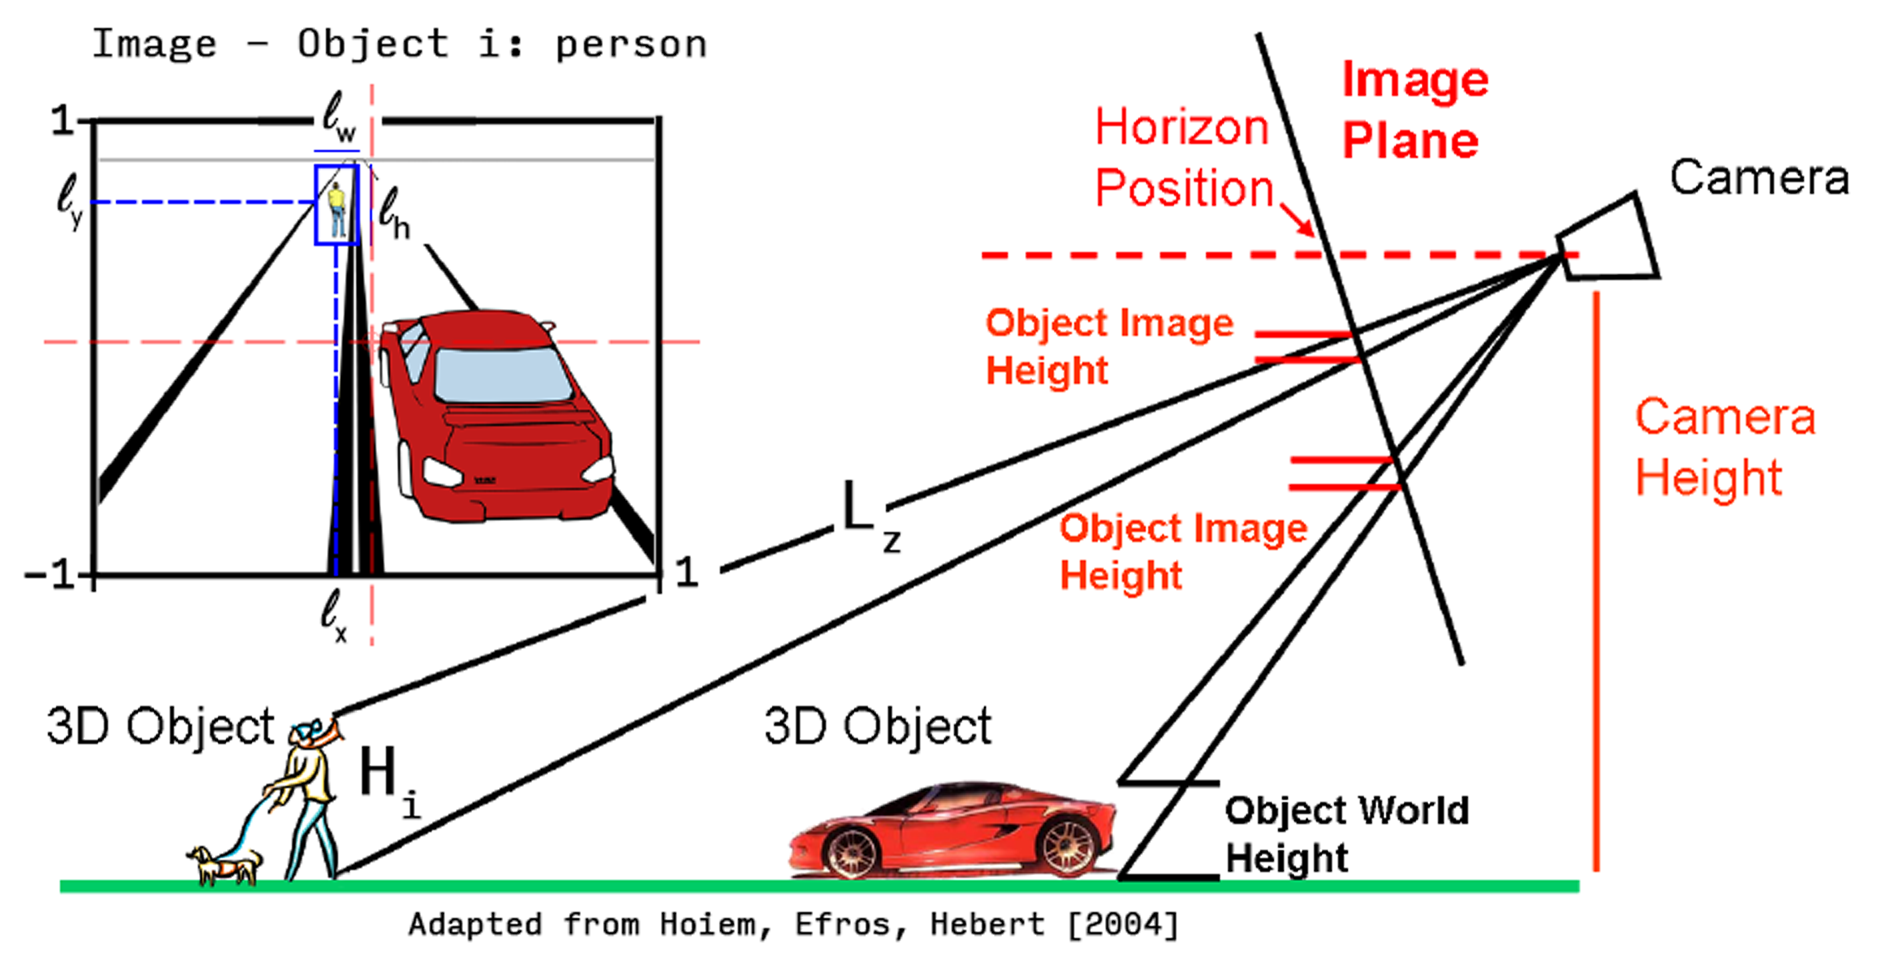
\includegraphics[width=14cm]{3DC.png}
			    \caption{Spatial coordinates\label{Hoeim}}
			\end{figure}
			The real world height of each category is pre-defined e.g.
			$H_{human}$:=1.7m, $H_{car}$:=1.5m.\\
			To handle the case where an object category $i$ has multiple instances in an image, we set $L_i$ to the median of all instances. Over the mean, the median is more robust to skewed distributions and would reflect the spatial arrangement of object categories.\\
			We take $L_z$ on a logarithmic scale since it's more heavily distributed around small values, and we drop the horizontal coordinate due to its high variance \cite{gist}.\\
			To infer the presence/location joint distribution, we assume $(L_y^{(i)})_i$, $(\log L_z^{(i)})_i$ are jointly Gaussians and that $\LL|\B$ inherits the binary prior tree structure. 
			\begin{equation}
				\p(\LL,\B)=\p(L_{root})\p(b_{root})\prod_i\p(b_i|b_{\pi_i})\p(L_i|L_{\pi_i},b_i,b_{\pi_i})
				\label{eq2}
			\end{equation}
			\begin{figure}[H]
			    \centering
			    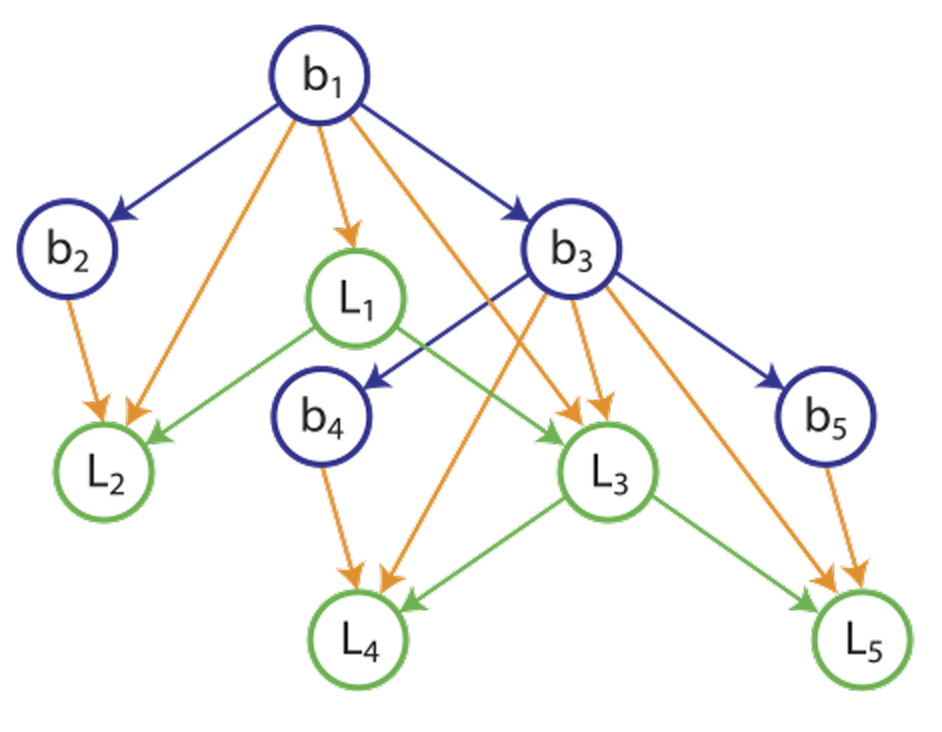
\includegraphics[width=6cm]{tree1.png}
			    \caption{The context model : Graphical representation\label{tree1}}
			\end{figure}
			To learn the parameters of the joint distribution in (\ref{eq2}) $\p(b_i|b_{\pi_i})$ is estimated by counting the co-occurrences of parent-child pairs, and for $\p(L_i|L_{\pi_i},b_i,b_{\pi_i})$ we distinguish three cases depending on the presence of the child object and its parent:
			\begin{equation}
			\p(L_i|L_{\pi_i},b_i,b_{\pi_i})=
			\begin{cases}
			\N(L_i|L_{\pi_i},\Sigma_{i}^{(1)})\text{ if }b_i=b_{\pi_i}=1\\
			\N(L_i|\mu_2^{(i)},\Sigma_{i}^{(2)})\text{ if }b_i=1,\:b_{\pi_i}=0\\
			\N(L_i|\mu_3^{(i)},\Sigma_{i}^{(2)})\text{ if }b_i=0
			\end{cases}
			\end{equation}
	\subsection{Measurement model:}
		This part of the framework includes, for a given image, a global feature vector namely the gist descriptor $g$ (\cite{gist}) summing up the overall statistics of the scene. The measurement model also integrates single-object detectors outputs.
		\subsubsection{Gist descriptors:}
			We train $\p(g|\B)$ using the gist descriptors of the images in our training set, so that we can characterise a type of scenes (containing a typical set of objects) with a particular gist descriptor. For this task we fit $\p(b_i|g)$ with logistic regression for each object category $i$ and retrieve $\p(g|b_i)$ using Bayes' rule.
			
		\subsubsection{Baseline detectors:}
			For an object category $i$, a local detector  yields a set of candidate windows $\{W_{i,k}\}_{1\leq k\leq K_i}$ each with a score (confidence) $s_{i,k}$. We apply the same coordinates transformation as in (\ref{coord}) to the suggested windows and assess their correctness on a training set via the binary variables $c_{i,k}=\I\{\text{correct detection}\}$.  
			\begin{figure}[H]
			    \centering
			    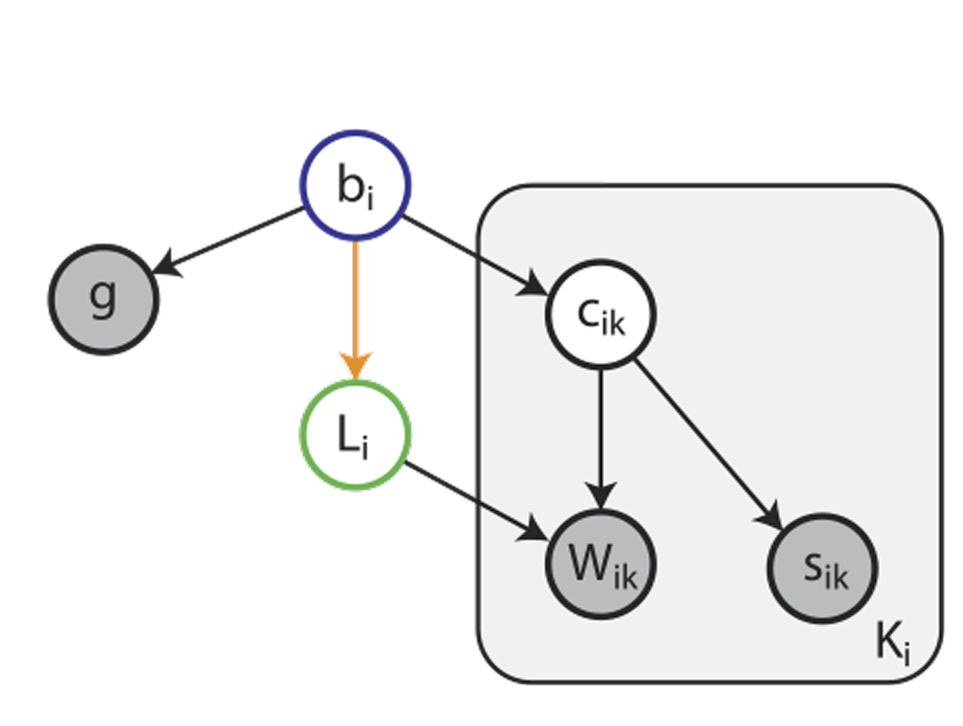
\includegraphics[width=6cm]{tree2.png}
			    \caption{The measurement model : Graphical representation\label{tree2}}
			\end{figure}
			The probability of correct detection $\p(c_{i,k}=1|b_i=1)$ is trained using the ground-truth labels and correct detections in the training set, and we set $\p(c_{i,k}=1|b_i=0)=0$. For the scores ${s_{i,k}}$ we use logistic regression once again to fit logistic regression to fit $\p(c_{i,k}|s_{i,k})$ and deduce $\p(s_{i,k}|c_{i,k})$.
			\\
			As for the candidate windows we assume:
			\begin{equation}
			\p(W_{i,k}|c_{i,k},L_i)=
			\begin{cases}
			\N(W_{i,k}|L_i,\Lambda_i)\text{ if }c_{i,k}=1\\
			const,\:\text{ otherwise}
			\end{cases}
			\end{equation}
			From the graphical models in figures (\ref{tree1},\ref{tree2}), we can rewrite the joint distribution as:
			\begin{equation}
			\begin{split}
			\p(\LL,\B)&=\p(L_{root})\p(b_{root})\prod_i\bigg(\p(b_i|b_{\pi_i})\p(L_i|L_{\pi_i},b_i,b_{\pi_i})\\
			&\times \prod\limits_{k=1}^{K_i}(\p(c_{i,k}|b_i)\p(W_{i,k}|c_{i,k},L_i)\p(s_{i,k}|c_{i,k})\bigg)\p(g|\B)
			\end{split}
			\label{factor}
			\end{equation}
	\subsection{Context model inference}
		Given the inputs $g$: the gist descriptor, $\W\equiv\{W_{i,k}\}_{i,k}$ and their respective score $\bS\equiv\{s_{i,k}\}_{i,k}$, we want to infer the binary variable $\B$ and $\C\equiv\{c_{i,k}\}_{i,k}$ and the expected locations $\LL$ by solving:
		\begin{equation}
		\hat \B,\hat \C,\hat \LL=\arg\max_{\B,\C,\LL} \p(\B,\C,\LL|g,\bS,\W)
		\end{equation}
		The exact inference being complicated we would solve this optimization problem by alternating between optimizing $\B,\C$ and optimizing the location $\LL$ that is:
		\begin{enumerate}[label=(\alph{*}), ref=(\alph{*})]
		\item Initialization\label{init}: $\hat \B,\hat \C=\arg\max\limits_{\B,\C}\p(\B,\C|g,\bS)$
		\item Location\label{gauss}: $\LL=\arg\max\limits_{\LL}\p(\LL|\hat\B,\hat\C,\W)$
		\item Presence\label{bin}: $\hat\B,\hat\C=\arg\max\limits_{\B,\C}\p(\B,\C|g,\bS,\hat\LL,\W)=\arg\max\limits_{\B,\C}\p(\B,\C|g,\bS)\p(\hat\LL,\W|\B,\C)$
		\end{enumerate}
		In the step \ref{init} we use Viterbi's algorithm (max-product) in the binary tree to compute the most probable $\B,\C$, given the parameters $g$ and $\bS$. For \ref{bin} we follow the same approach with the edges and nodes potentials being affected by the distributions of the location and measurement variables $\LL,\W|\hat \B,\hat \C$. This step could be interpreted as encouraging objects with favorable spatial arrangement to be present in the image.\\

		For step \ref{gauss}, we use the sum-product algorithm on the gaussian tree $\LL|\B,\C$. 

		In the experiment we use three iterations alternating between inference of $\B,\C$ and inference of $\LL$.

		We will use once again the sum-product algorithm this time on the binary tree $\B,\C|\LL$ to compute all the marginals, as well as the conditional marginals; specifically:
		\[
		\begin{split}&\p(b_i=1|\bS,g,\hat\LL,\W)\phantom{abc}\text{(Presence prediction tasks)}\\
		&\p(c_{i,k}=1|\bS,g,\hat \LL|,\W)\text{  (Localization tasks)}
		\end{split}\]

\section{Experiments}
	We apply the model above to object localization and presence predication on the SUN database\cite{sun}.
	The average object size is 5 percent of the image size, and a typical image contains seven different object categories which makes this database suitable for leveraging contextual information.

	We divide this database into a training set of 4367 images and a test set of 4317 images presenting 111 object categories.

	We use the MATLAB Toolbox for the LabelMe Image Database \cite{LM} to handle the SUN images, objects and different attributes as well as to compute the gist descriptor.

	In Matlab we learn the co-occurrences tree using Prim's algorithm to find the maximum weight spanning tree
	in 1.6s of which 4ms to find the MST. In fact, the chosen structure is very sparse as it considers only pairs of objects which makes the model scalable. And the results (figure ) shows that this hierarchy is natural and summarizes succinctly the objects dependencies.

	Since the output of the Chow-Liu algorithm is an undirected tree, we root the tree at an arbitrary node (e.g. \texttt{sky}).

	Out of the 110 edges of the tree, 86 (78\%) have positive weights; which means that the database is rich with objects pairs that occur quite often.

	\begin{figure}[H]
    \centering
    \subfloat[subtree \texttt{floor}]{
    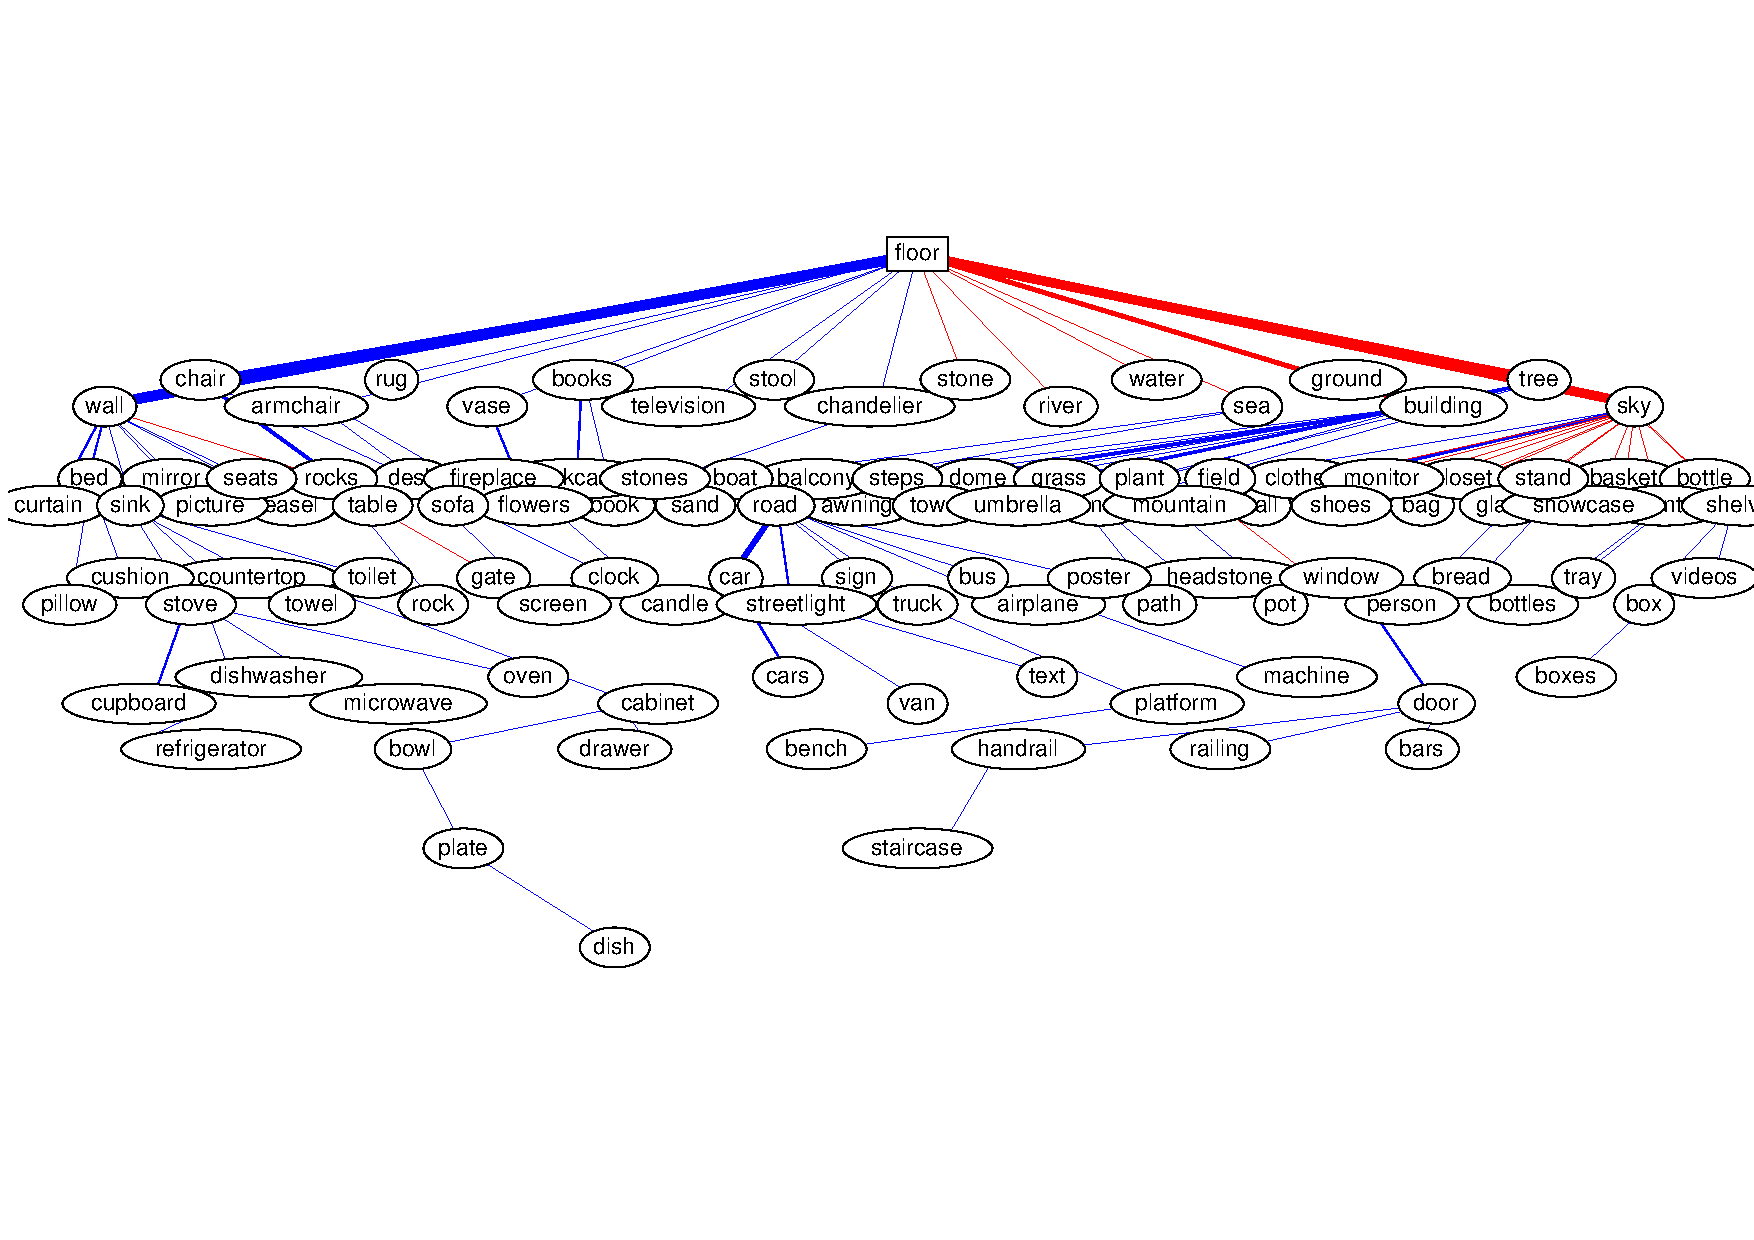
\includegraphics[width=16cm]{tree_floor.pdf}}
    \\
    \subfloat[subtree \texttt{sky}]{
    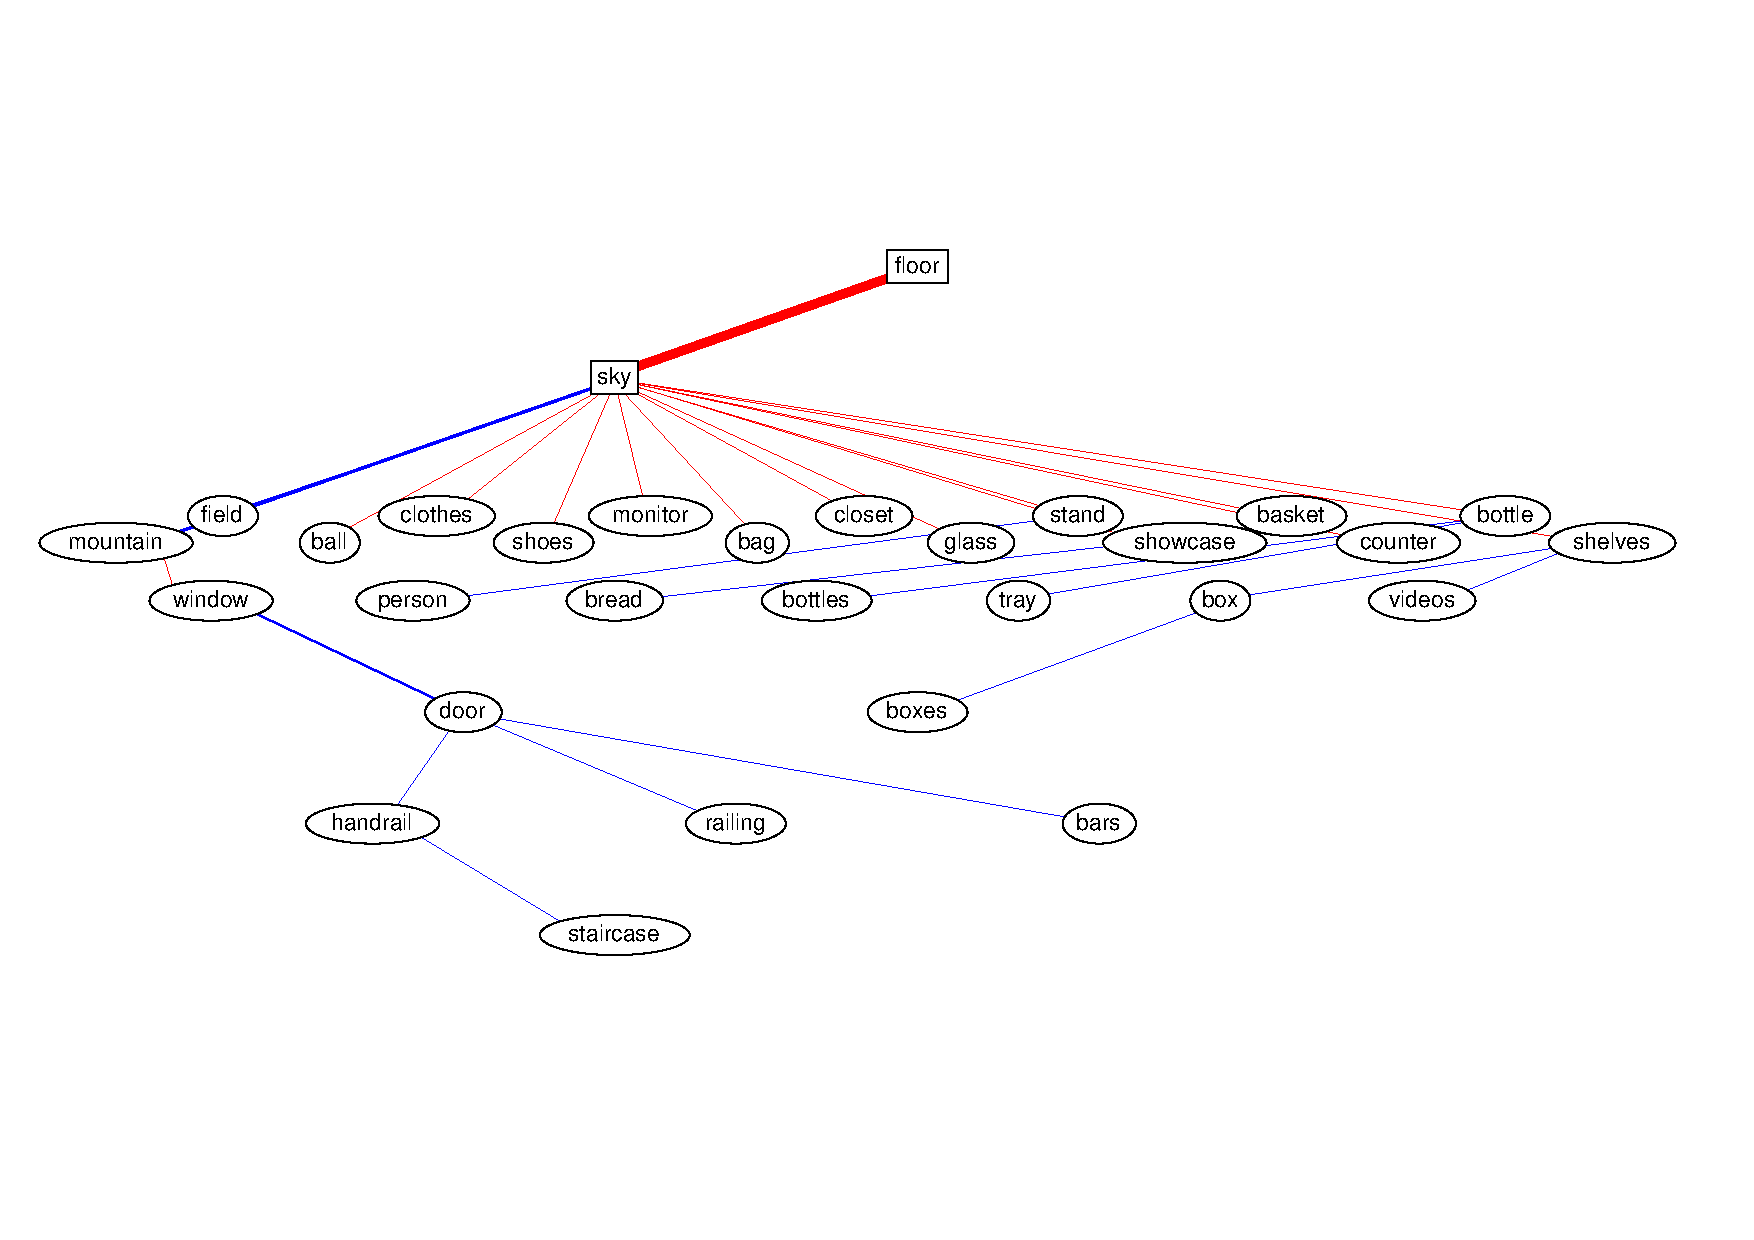
\includegraphics[width=16cm]{tree_sky.pdf}}
    \caption{Subtrees of the co-occurrences hierarchy\\ \textcolor{red}{Red} : negative correlations - \textcolor{blue}{Blue}: positive correlations\\ The thickness of each edge is proportional to the strength of the correlation.}
	\end{figure}
	We note that some objects (e.g. floor) divide the tree according to the scene category

	To assess the model's performance at interpreting the scenes we show the percentage of images in which the top N most confident detections are all correct (for both presence prediction and localization).
	\begin{figure}[H]
    \centering
    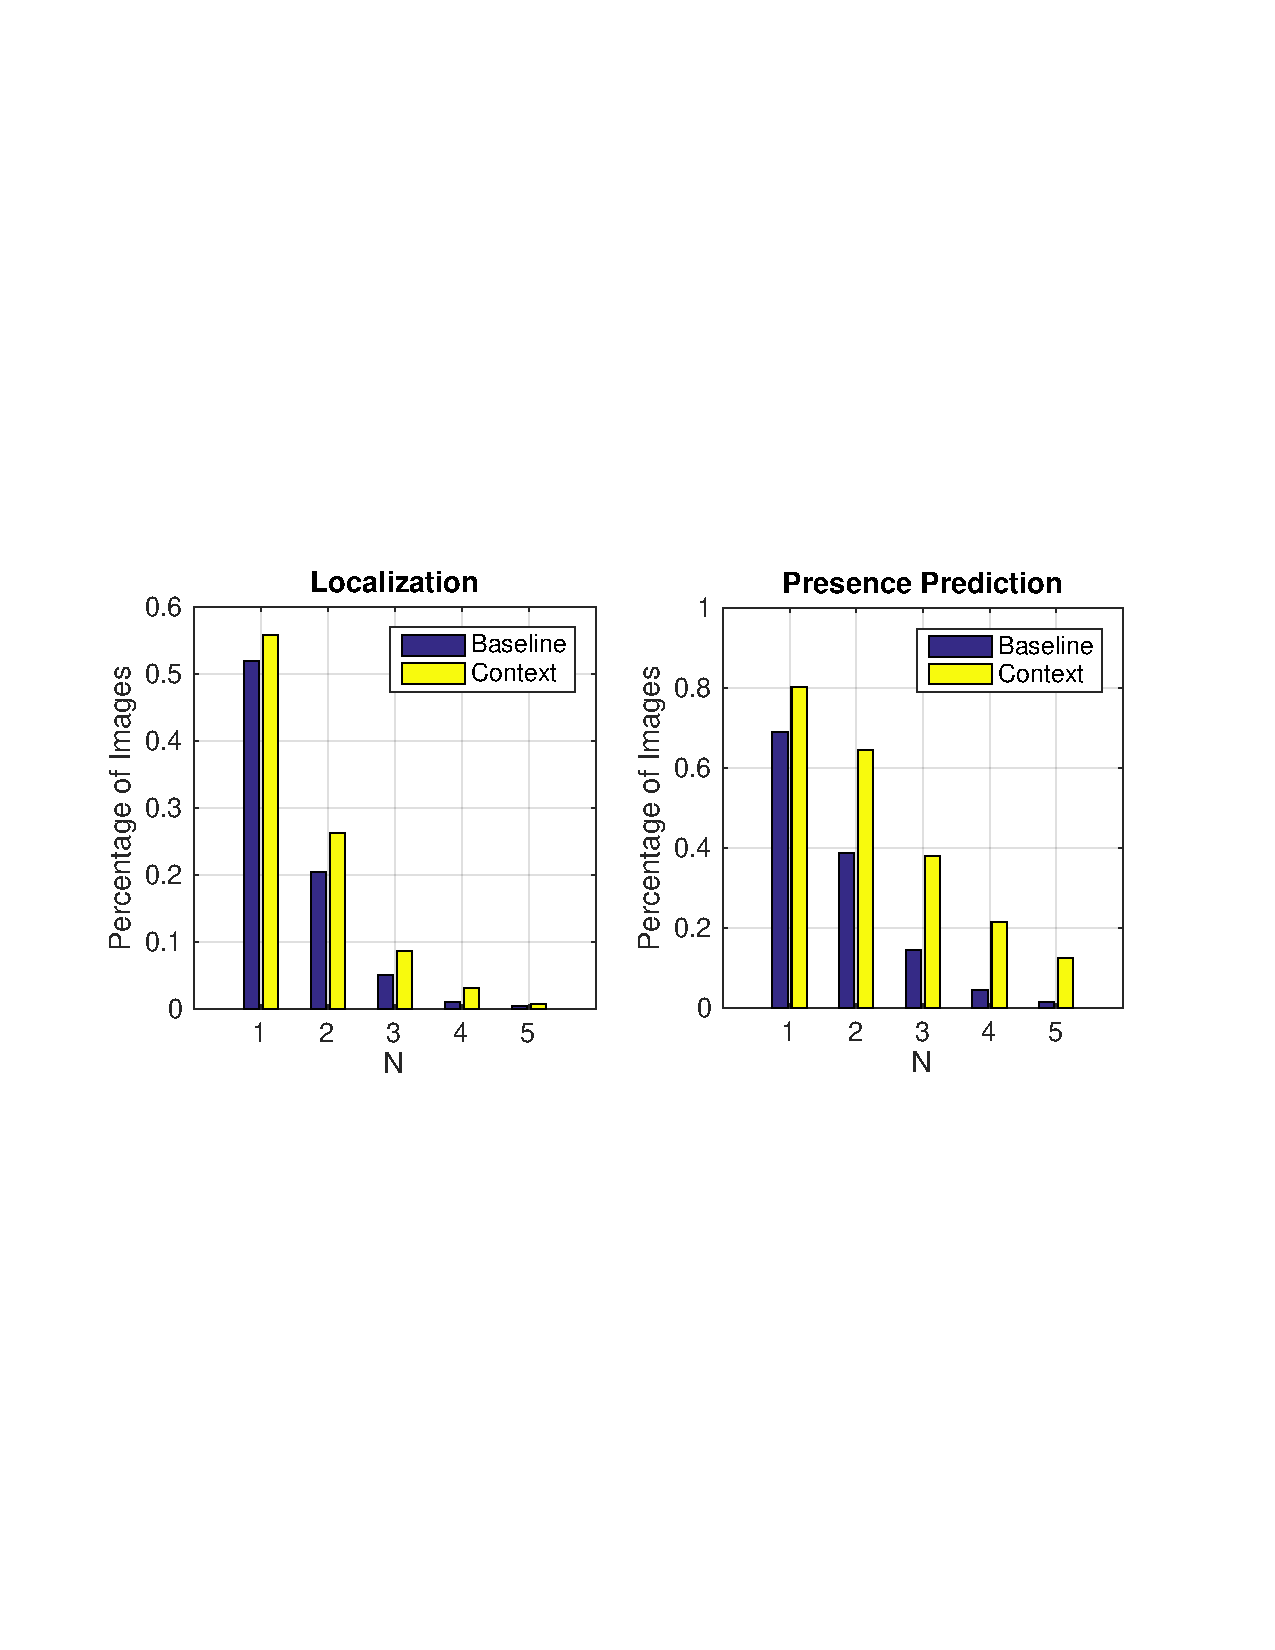
\includegraphics[width=12cm]{topN}
    \caption{top N most confident detections}
	\end{figure}

	The inference of the model parameters as detailed above takes around 0.34s per image. We compare the average precision for object localization (Table \ref{aploc}) and presence prediction (Table \ref{appr}) with and without the context model. We note that generally the model achieves its objective, that is, to enhance the scores of the bounding boxes proposed by the baseline detectors. Out of 111 object categories we improved the presence detection performance of 102 classes, but only 72 for the localization.
	\begin{figure}[H]
    \centering
	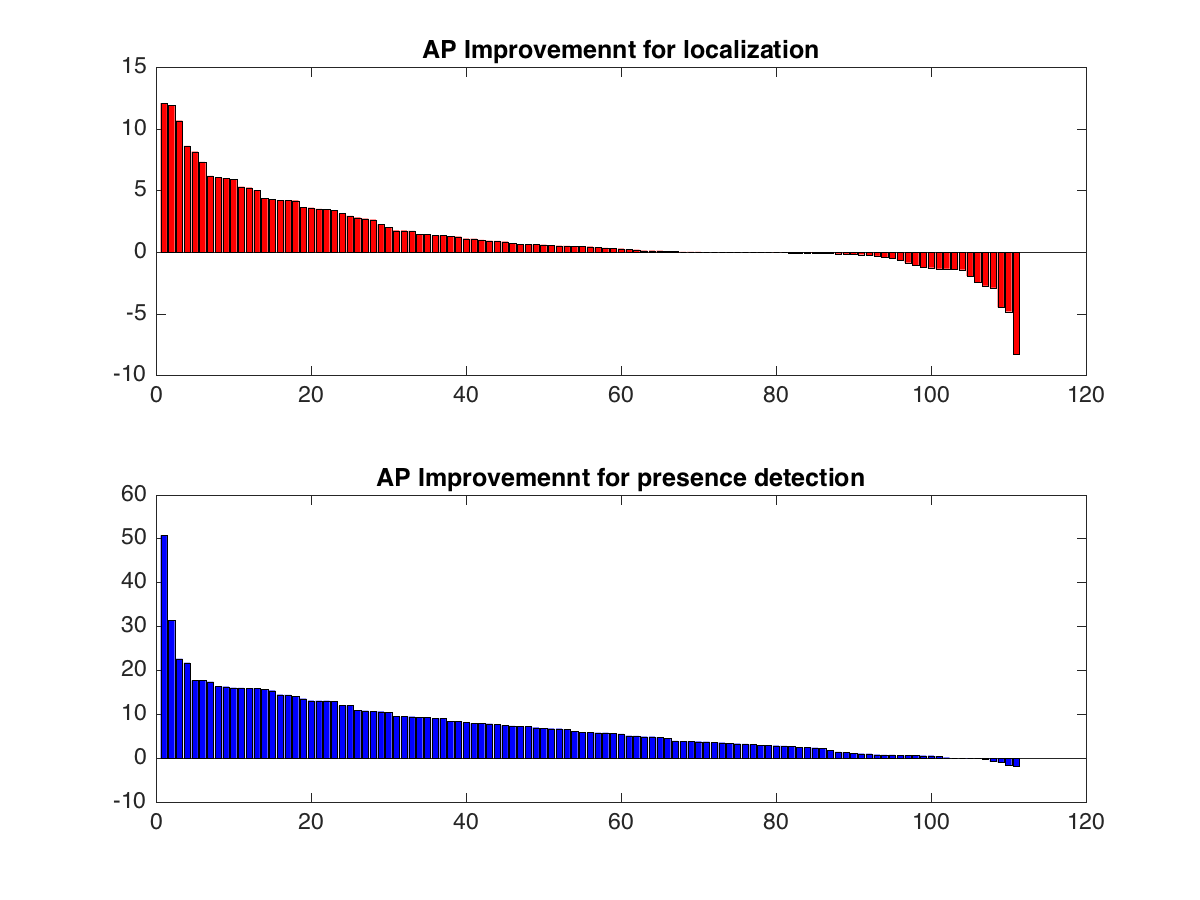
\includegraphics[width=15cm]{improv}
	\caption{Average precision improvement with the context}
	\end{figure}
	\begin{figure}[H]
    \centering
    \subfloat[Presence prediction]{
    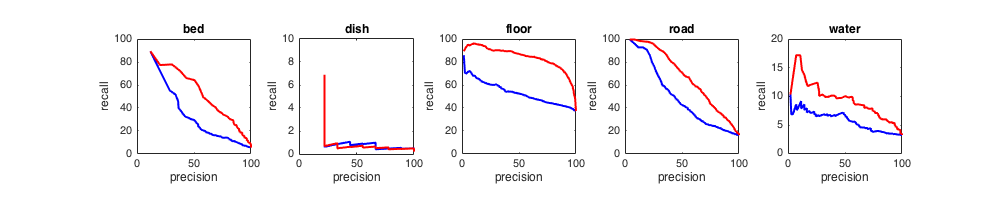
\includegraphics[width=18cm]{pres1}}
    \\
	\subfloat[Localization]{
    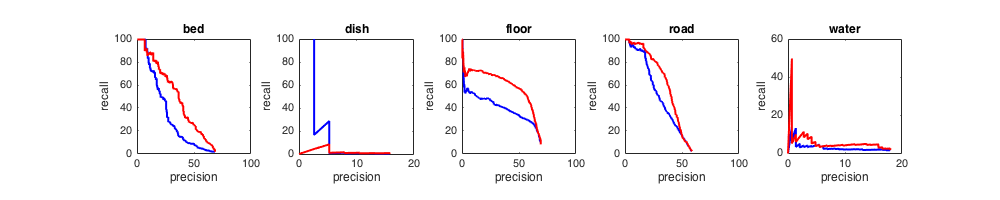
\includegraphics[width=18cm]{loc1}}
    \caption{Precision-recall curves: red(context) vs blue(baseline)\label{roc}}
	\end{figure}
	In the precision recall curves of figure (\ref{roc}), 2 out 5 classes have their localization performances deteriorated with the context model of which 1 (\texttt{dish} : leaf node) hasn't been improved in the presence detection task as well.

	We note that non-leaf nodes act as if they are representing scene categories and the performance on theses classes benefit from the context integration as opposed to the classes with higher level (distance to the root). 

%--------------------------------------------
%    				Biblio
%--------------------------------------------

\begin{thebibliography}{2}
\bibitem{htree} Choi, M. J., Torralba, A., \& Willsky, A. S. (2012). A tree-based context model for object recognition. Pattern Analysis and Machine Intelligence, IEEE Transactions on, 34(2), 240-252.

\bibitem{3D}Hoiem, D., Efros, A. A., \& Hebert, M. (2008). Putting objects in perspective. International Journal of Computer Vision, 80(1), 3-15.

\bibitem{gist}Torralba, A. (2003). Contextual priming for object detection. International journal of computer vision, 53(2), 169-191.

\bibitem{LM} B. C. Russell, A. Torralba, K. P. Murphy, W. T. Freeman (2008). LabelMe: a database and web-based tool for image annotation. International Journal of Computer Vision on, 77(1-3), 157-173.

\bibitem{SUN} SUN Database: Large-scale Scene Recognition from Abbey to Zoo". J. Xiao, J. Hays, K. Ehinger, A. Oliva, and A. Torralba. IEEE Conference on Computer Vision and Pattern Recognition, 2010.
\end{thebibliography}

\appendix
	\begin{table}[H]
	\centering
	\begin{tabular}{|c|c|c||c|c|c||c|c|c|}
	\hline
	Category & baseline & context & Category & Baseline & Context & Category & Baseline & Context\\
	\hline
		airplane & 35.11 & 33.17 & armchair & 9.62 & 10.97 & awning & 1.52 & 0.11 \\
		bag & 0.28 & 0.04 & balcony & 3.06 & 1.71 & ball & 9.09 & 9.09 \\
		bars & 0.03 & 0.37 & basket & 9.15 & 9.16 & bed & 26.27 & 36.92 \\
		bench & 0.04 & 0.03 & boat & 0.08 & 0.13 & book & 0.03 & 0.10 \\
		bookcase & 2.32 & 4.95 & books & 1.46 & 3.21 & bottle & 4.60 & 5.11 \\
		bottles & 0.01 & 0.35 & bowl & 0.90 & 3.15 & box & 0.19 & 0.12 \\
		boxes & 3.03 & 9.09 & bread & 0.20 & 0.10 & building & 14.38 & 15.82 \\
		bus & 9.13 & 9.35 & cabinet & 0.43 & 1.87 & candle & 0.25 & 0.05 \\
		car & 15.92 & 16.54 & cars & 0.00 & 0.02 & chair & 11.64 & 12.55 \\
		chandelier & 18.30 & 22.68 & clock & 9.09 & 9.09 & closet & 1.13 & 9.28 \\
		clothes & 0.26 & 0.54 & counter & 0.10 & 0.22 & countertop & 0.18 & 1.17 \\
		cupboard & 5.30 & 9.49 & curtain & 6.62 & 10.80 & cushion & 6.11 & 9.60 \\
		desk & 0.76 & 3.56 & dish & 9.15 & 0.86 & dishwasher & 20.45 & 24.05 \\
		dome & 10.61 & 9.52 & door & 8.01 & 6.75 & drawer & 1.70 & 2.36 \\
		easel & 0.00 & 0.00 & fence & 0.19 & 1.04 & field & 19.77 & 24.99 \\
		fireplace & 7.66 & 5.22 & floor & 31.34 & 43.42 & flowers & 0.20 & 1.54 \\
		gate & 0.91 & 1.30 & glass & 0.17 & 0.10 & grass & 11.04 & 12.34 \\
		ground & 1.49 & 2.05 & handrail & 0.88 & 0.58 & headstone & 0.14 & 0.14 \\
		machine & 9.10 & 9.10 & microwave & 27.71 & 31.93 & mirror & 0.83 & 5.13 \\
		monitor & 4.07 & 3.21 & mountain & 17.23 & 18.95 & oven & 8.07 & 13.37 \\
		path & 0.59 & 1.85 & person & 17.66 & 17.02 & picture & 1.65 & 2.39 \\
		pillow & 9.13 & 9.32 & plant & 1.10 & 4.75 & plate & 1.55 & 0.35 \\
		platform & 0.01 & 0.02 & poster & 0.32 & 0.31 & pot & 9.15 & 9.12 \\
		railing & 9.09 & 9.09 & refrigerator & 6.14 & 18.06 & river & 2.90 & 5.61 \\
		road & 33.20 & 39.09 & rock & 0.20 & 0.13 & rocks & 0.45 & 0.26 \\
		rug & 0.15 & 0.65 & sand & 3.95 & 4.42 & screen & 9.57 & 10.08 \\
		sea & 28.66 & 33.67 & seats & 1.85 & 9.16 & shelves & 2.58 & 4.33 \\
		shoes & 0.05 & 0.01 & showcase & 0.03 & 0.62 & sign & 0.57 & 0.15 \\
		sink & 2.11 & 5.05 & sky & 55.34 & 61.35 & sofa & 11.47 & 14.87 \\
		staircase & 4.57 & 1.84 & stand & 0.27 & 1.35 & steps & 0.65 & 0.17 \\
		stone & 0.00 & 0.12 & stones & 1.52 & 0.16 & stool & 10.78 & 11.88 \\
		stove & 9.88 & 10.32 & streetlight & 3.17 & 9.34 & table & 9.84 & 10.76 \\
		television & 11.94 & 10.51 & text & 9.09 & 9.09 & toilet & 22.01 & 19.12 \\
		towel & 4.61 & 4.63 & tower & 1.29 & 1.15 & tray & 0.48 & 9.09 \\
		tree & 10.88 & 12.89 & truck & 9.65 & 4.83 & umbrella & 0.22 & 0.08 \\
		van & 10.26 & 5.80 & vase & 0.20 & 0.84 & videos & 2.27 & 2.39 \\
		wall & 14.70 & 17.85 & water & 1.51 & 5.01 & window & 9.95 & 9.94 \\
	\hline
	\hline
	&&&\textbf{Average} & \textbf{6.82} &  \textbf{8.10} &&&\\
	\hline
	
	\end{tabular}
	\caption{Localization average precision per category\label{aploc}}
	\end{table}

	\begin{table}[H]
	\centering
	\begin{tabular}{|c|c|c||c|c|c||c|c|c|}
	\hline
	Category & baseline & context & Category & Baseline & Context & Category & Baseline & Context\\
	\hline
		airplane & 36.96 & 47.54 & armchair & 9.15 & 18.43 & awning & 2.67 & 9.61 \\
		bag & 2.83 & 5.64 & balcony & 5.76 & 9.27 & ball & 1.64 & 3.43 \\
		bars & 1.04 & 9.40 & basket & 4.56 & 8.09 & bed & 37.77 & 55.42 \\
		bench & 3.24 & 3.34 & boat & 3.03 & 8.06 & book & 2.26 & 8.97 \\
		bookcase & 11.72 & 20.78 & books & 10.29 & 20.90 & bottle & 10.01 & 15.93 \\
		bottles & 1.24 & 4.46 & bowl & 5.88 & 10.76 & box & 6.46 & 13.15 \\
		boxes & 4.20 & 7.54 & bread & 2.30 & 6.19 & building & 55.95 & 71.90 \\
		bus & 3.20 & 3.89 & cabinet & 7.42 & 15.85 & candle & 2.52 & 3.27 \\
		car & 42.83 & 65.45 & cars & 2.92 & 53.64 & chair & 37.73 & 47.27 \\
		chandelier & 16.74 & 24.23 & clock & 5.68 & 4.00 & closet & 6.58 & 7.02 \\
		clothes & 2.08 & 5.37 & counter & 3.20 & 5.44 & countertop & 5.58 & 11.31 \\
		cupboard & 18.11 & 34.10 & curtain & 22.66 & 35.69 & cushion & 4.91 & 14.34 \\
		desk & 11.69 & 22.56 & dish & 2.44 & 2.34 & dishwasher & 13.11 & 22.61 \\
		dome & 5.61 & 9.40 & door & 30.34 & 37.57 & drawer & 4.13 & 7.05 \\
		easel & 0.90 & 1.62 & fence & 7.04 & 23.41 & field & 35.16 & 49.26 \\
		fireplace & 3.07 & 3.60 & floor & 51.27 & 82.61 & flowers & 6.65 & 14.30 \\
		gate & 2.27 & 3.32 & glass & 4.13 & 4.79 & grass & 21.67 & 37.58 \\
		ground & 12.90 & 17.76 & handrail & 6.10 & 6.74 & headstone & 0.56 & 0.56 \\
		machine & 1.01 & 0.96 & microwave & 22.36 & 27.83 & mirror & 6.29 & 19.33 \\
		monitor & 5.05 & 4.05 & mountain & 55.40 & 63.31 & oven & 7.41 & 15.21 \\
		path & 5.46 & 11.14 & person & 53.37 & 59.51 & picture & 9.51 & 10.79 \\
		pillow & 5.75 & 23.40 & plant & 24.77 & 34.02 & plate & 2.80 & 7.33 \\
		platform & 0.69 & 0.68 & poster & 3.77 & 4.77 & pot & 8.60 & 11.04 \\
		railing & 4.50 & 5.05 & refrigerator & 7.82 & 23.19 & river & 5.91 & 22.17 \\
		road & 49.41 & 66.77 & rock & 2.61 & 5.03 & rocks & 5.96 & 8.28 \\
		rug & 3.04 & 12.09 & sand & 8.55 & 22.93 & screen & 9.54 & 17.47 \\
		sea & 38.51 & 50.50 & seats & 4.49 & 16.46 & shelves & 12.95 & 23.71 \\
		shoes & 1.09 & 1.69 & showcase & 1.09 & 9.25 & sign & 6.99 & 22.88 \\
		sink & 14.38 & 36.08 & sky & 78.28 & 91.19 & sofa & 15.25 & 18.94 \\
		staircase & 8.06 & 9.45 & stand & 4.71 & 7.43 & steps & 5.53 & 10.60 \\
		stone & 2.75 & 9.28 & stones & 2.20 & 12.63 & stool & 10.00 & 10.98 \\
		stove & 18.87 & 31.93 & streetlight & 13.32 & 19.13 & table & 26.37 & 39.90 \\
		television & 9.14 & 7.23 & text & 5.13 & 9.86 & toilet & 41.21 & 45.07 \\
		towel & 4.37 & 11.58 & tower & 4.34 & 3.61 & tray & 3.21 & 5.97 \\
		tree & 67.83 & 74.61 & truck & 11.46 & 14.37 & umbrella & 1.52 & 1.36 \\
		van & 9.24 & 23.67 & vase & 3.63 & 10.95 & videos & 2.90 & 6.03 \\
		wall & 67.72 & 83.45 & water & 6.19 & 9.93 & window & 52.30 & 58.04 \\
	\hline
	\hline
	&&&\textbf{Average} & \textbf{13.38} &  \textbf{20.73} &&&\\
	\hline
	\end{tabular}
	\caption{Presence prediction average precision per category\label{appr}}
	\end{table}



\end{document}
